%---------------------------------------------------------------------------------
%                西南交通大学研究生学位论文:第二章内容
%---------------------------------------------------------------------------------
\chapter{网络编码和TCP/NC协议}
本章主要介绍网络编码基础原理,重点分析了线性网络编码。详细说明了TCP/NC协议的设计原理。
\section{网络编码理论基础}
2000年,R. Ahlswede等在论文“Network Information Flow”\textsuperscript{\cite{Ahlswede2000}}中创造性地提出了“网络编码”新概念,首次将编码和路由有机地结合在一起,建立了一种全新的网络体系结构,不仅解决了广播路由这一信息论中的经典难题,而且使得达到组播网络容量的理论上限成为可能。
网络编码建立在一个简单而广泛的概念的基础上:在包交换网络中,中间节点不仅仅是简单地路由转发接收到的数据包,而是对它们进行一些函数操作并计算、转发操作结果\textsuperscript{\cite{梅达尔2014网络编码基础与应用}}。运用网络编码可以提高网络吞吐率、均衡网络负载和提高网络带宽利用率等。
\subsection{Network Coding基本概念}
我们以文献\cite{Ahlswede2000}中著名的蝶形网络,即图\ref{BUTTER_EPS},为例来说明Network Coding的基本原理。
\begin{figure}[htbp]
	\centering
	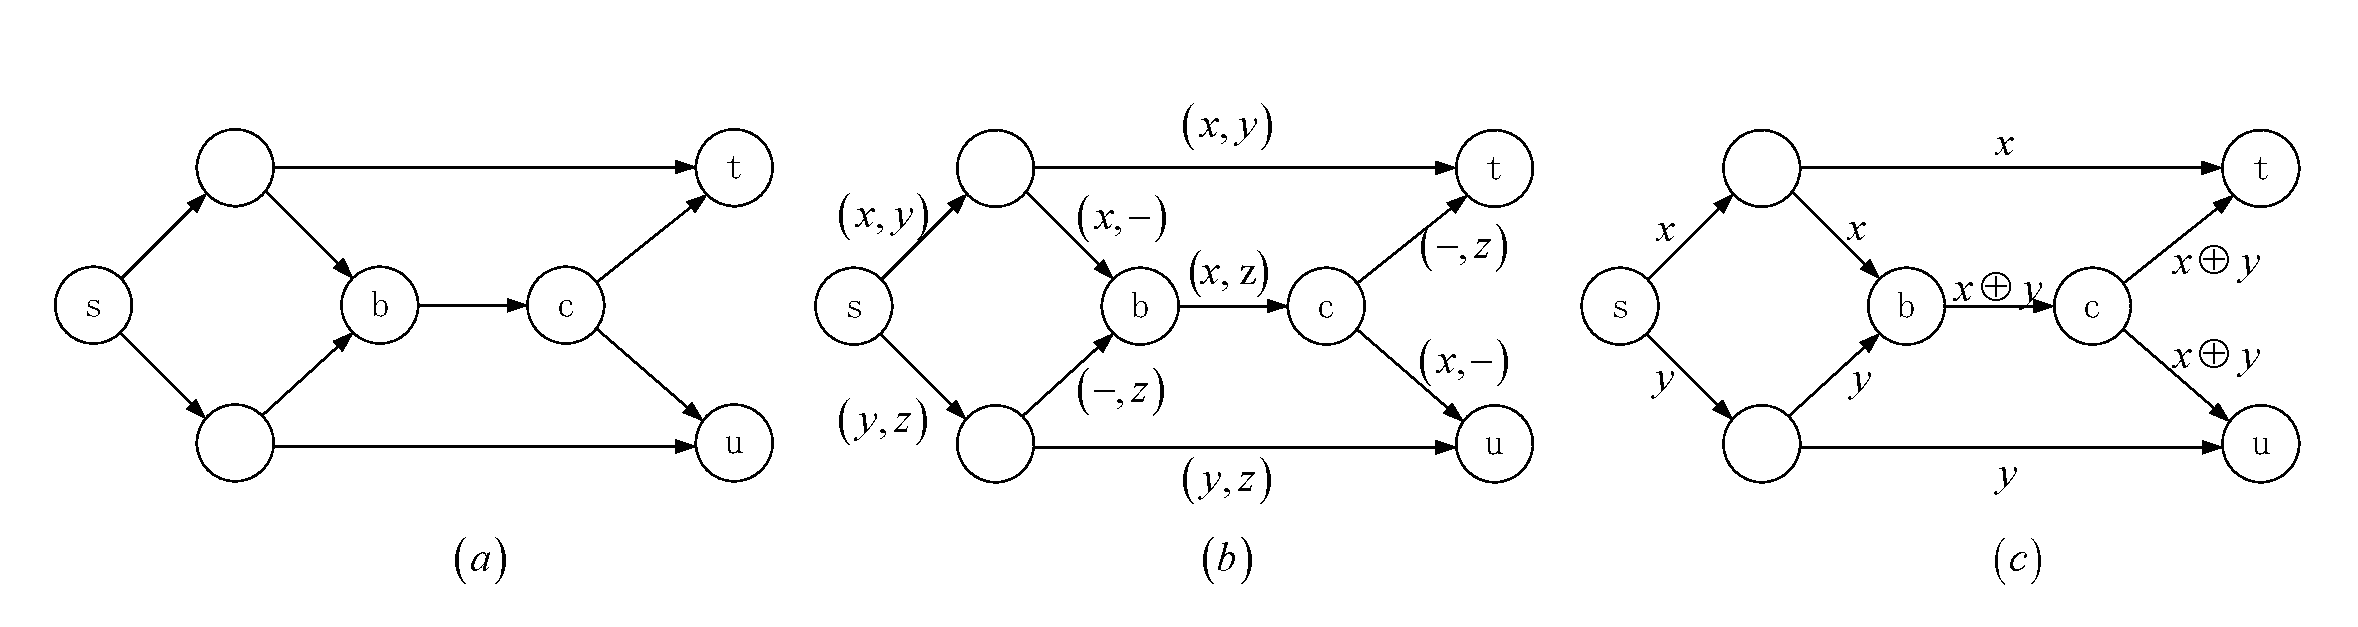
\includegraphics[width=6in]{figures/butter.eps}
	\caption{蝶形网络}
	\label{BUTTER_EPS}
\end{figure}
\par
图\ref{BUTTER_EPS}为一个包交换模型。在该网络中,源节点$s$需要将信息多播给两个目的的节点$t$和$u$。有向图的每一条有向边代表一条无差错包传输信道,每个 $channel\ use$可以传输1个长为$m$比特的数据包。源节点希望以尽可能高的速率与两个目的节点通信。
\par
解决该问题,传统的路由方法如图\ref{BUTTER_EPS}$(b)$为例。在第一个时隙内,源节点$s$将$x$发送给$t$和$u$,将$y$发送给$u$。在第二个时隙内,源节点$s$将$y$传给了$t$,将$z$传给了$t$和$u$。两个时隙结束后,两个目的节点$t$和$u$都收到了$x$,$y$,$z$这三个数据包。可以看到,使用传统的路由方法,在两个时隙内可以传输3个不同的报文给$t$和$u$,因此传统路由方法的多播吞吐量为$\dfrac{3}{2} packet/channel\ use$。该多播吞吐量已被证明是使用路由方法能够实现的最大吞吐量。
\par
然而使用图\ref{BUTTER_EPS}$(c)$所示的网络编码方法,能够实现$2\ packet/per channel\ use$。该方法中,第一个时隙源节点$s$仍分发两个数据包$x$和$y$,与路由方法不同的是,节点$b$将对$x$和$y$进行异或运算,并转发运算结果。目的节点$t$收到数据包$x$和$x\oplus y$,并根据它们恢复出$x$和$y$。同样地,目的节点$u$也可以恢复出$x$和$y$。网络编码以网络中间节点的编码操作和目的节点的解码操作为代价,提升了网络的多播吞吐量,并突破了路由方法所能实现的吞吐量上限。是否有能比图\ref{BUTTER_EPS}$(c)$更好的方案?答案是没有。一个网络的最大多播吞吐量取决于分割源节点和目的节点的最小割集\textsuperscript{\cite{Ahlswede2000}}。图\ref{BUTTER_EPS}$(a)$的最小割集为2,故图\ref{BUTTER_EPS}$(c)$已经是最优方案。
\par
从上述例子中我们可以明白,要想充分利用通信网络的信息传输容量,光靠改进路由算法是不够的。在网络中,多个信息数据包可以通过多种方式有效地结合在一起,目的节点再从这些结合后的信息中恢复出原来数据包,达到提高网络的吞吐率的目的。
\subsection{网络编码的图论模型}
一个组合包网络$N=(V,E,S,T,A)$包括:
\begin{enumerate}[fullwidth,itemindent=2em,label=(\arabic*)]
	\item 有限有向无环多重图$G=(V,E)$,其中$V$表示图$G$的顶点集合,$E$表示图$G$的有向边的多重集合。
	\item 无重复源节点集合$S \subset V$,$S = \left\{ {{s_1},{s_2}, \cdots ,{s_{\left| S \right|}}} \right\}$。
	\item 无重复目的节点集合$T \subset V$,$T = \left\{ {{t_1},{t_2}, \cdots ,{t_{\left| T \right|}}} \right\}$。
	\item 有限的数据包集合$A$,$\left| A \right| \ge 2$。
\end{enumerate}
\par
图$G$的顶点代表包交换网络中的通信节点,有向边代表通信节点之间的无差错传输信道。有向边$(u,v)$具有单位容量,即每条边每次只能将一个数据包( 从符号集$A$中选取的一个符号)从$u$传送给点$v$。如果要进行更大容量的传输,可以在$u$和$v$之间建立多条平行边,单位容量都为1。以图\ref{TULUNMOXING_EPS}单源多宿网络为例,图\ref{TULUNMOXING_EPS}$\left(b\right)$与图\ref{TULUNMOXING_EPS}本质上是一样的,仅仅是将所有的路径都转换为单位容量。对于顶点$u,v \in V$,如果$v=u$或者图$G$中存在一条从$u$到$v$的有向路径,就称$u$可达$v$。在有向边$\left(u,v\right) \in E$上进行的操作是将点$u$发出的数据包$p \in A$无差错地交付给点$v$。
\begin{figure}[htbp]
	\centering
	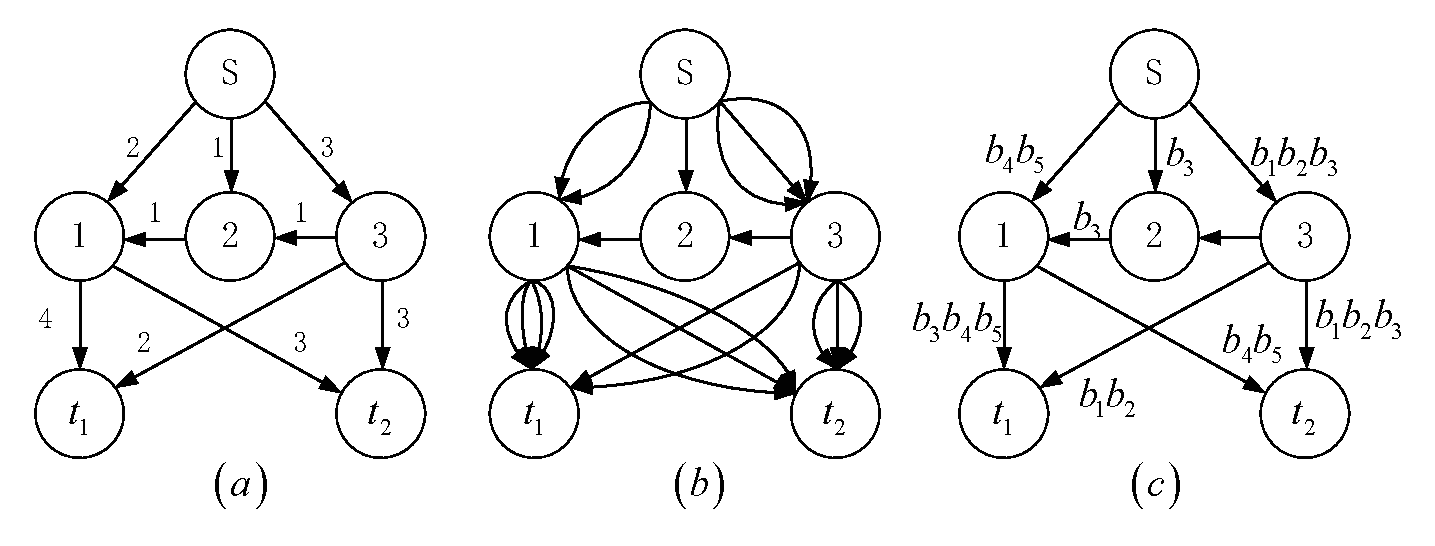
\includegraphics[width=6in]{figures/tulunmoxing.eps}
	\caption{单源多宿网络( 没有网络编码)}
	\label{TULUNMOXING_EPS}
\end{figure}
\par
对于顶点$v \in V$,我们用$I\left( v \right)$表示所有进入点$v$的边的集合,用$O\left( v \right)$表示所有从点$v$出发的边的集合。那么,组合包网络中的组合逻辑指的是:顶点$v$的出边集合$O\left( v \right)$中的任一非空闲边上传输的数据包是来自其入边集合$I\left( v \right)$中的所有非空闲数据包经过$v$的编码函数处理后得到的数据包集合。对于一个实际网络而言,在节点$v$通过某个数据包函数对入边集合的数据包进行处理,生成输出数据包之前,进入节点的数据包是需要被缓存的。
\par
节点$v$使用的函数被称为$v$的本地编码函数。当$v$只有路由功能时,它的出边上发送的数据包可以看做是对入边上收到的数据包的复制,即图\ref{TULUNMOXING_EPS}$\left( c \right)$所示的情况。图\ref{TULUNMOXING_EPS}$\left(c\right)$中,网络内部节点$1,2,3$仅仅通过存储转发的方法就达到了多播最大吞吐率,即源节点$s$可以同时发送5个数据包$b_{1}b_{2}b_{3}b_{4}b_{5}$给$t_{1}$和$t_{2}$。当$v$具有对入边数据包进行编码的功能后,如图\ref{BUTTER_EPS}$\left(c\right)$中节点$b$所示,网络多播吞吐率突破了仅仅使用路由方法的吞吐率上限。
\par
\par
网络编码的基本思想是对进入节点的所有数据包进行更一般性的本地编码操作,而不仅仅是简单地复制,从而获得性能上的增益。

\subsection{线性网络编码}\label{xianxingbianma}
在阐述线性网络编码之前,先简单介绍近世代数的相关概念。
\begin{myDef}[群]
	对于一个非空元素集合$G$以及定义在$G$上的一种运算“$*$”( 这里的$*$泛指一种代数运算,如$+$,$-$,$\times$,$\div$,模$m$加$\oplus$,模$m$乘$\odot$等)。若满足以下四个条件:
	\begin{enumerate}[fullwidth,itemindent=2em,label=(\arabic*)]
		\item 封闭性,即$\forall a,b \in G$,$\exists\left(a*b\right)=c\in G$。
		\item 结合性,即$\forall a,b \in G$,$\exists a*\left(b*c\right)=\left(a*b\right)*c$。
		\item 存在唯一一个单位元$e$,即$\forall a \in G$,$\exists a*e=e*a=a$。
		\item $G$中的每个元素各自存在唯一的逆元,即$\forall a \in G$,$\exists {a^{ - 1}} \in G$,使得$a*{a^{-1}}={a^{-1}}*a=e$。这里${a^{-1}}$泛指逆元。
	\end{enumerate}
\par
则称这样的代数系统为群,记做$\left(G,*\right)$。
\end{myDef}
\begin{myDef}[交换群]
	如果一个群满足交换律,即$\forall a,b \in G$,$\exists a*b=b*a$,则称这样的代数系统为交换群,也叫阿贝尔群。
\end{myDef}
\par
如果群$\left(G,*\right)$中的运算$*$是加法,则称群$\left(G,+\right)$为加群。加群一定是交换群。加群中一定包含零元素,零元素正是该加群的单位元$e$,加群元素$a$的逆元$a^{-1}$是代数中的$-a$。
\begin{myDef}[环]
	对于非空元素的集合$R$以及定义在$R$上的乘、加两种运算,如满足以下3个条件:
	\begin{enumerate}[fullwidth,itemindent=2em,label=(\arabic*)]
		\item 集合$R$在加运算可构成加群$\left(R,+\right)$。
		\item 集合$R$在乘运算下满足群的前三个条件,即封闭性、结合性和单位元存在性
		\item 分配率,即$\forall a,b,c \in R$,$\exists a \cdot \left(b+c\right)=a \cdot b + a \cdot c$,$\left(b+c\right) \cdot a=b \cdot a + c \cdot a$。
	\end{enumerate}
\par
则称这样的代数系统为环。
\end{myDef}
\begin{myDef}[交换环]
	如果环满足乘法交换律,即$\forall a,b \in R$,$\exists a \cdot b=b \cdot a$。称该环为交换环。
\end{myDef}
\begin{myDef}[域]
	对于至少含有一个非零元素的交换环,若每个非零元素都存在乘运算下的逆元,则称该交换环为域,记做$\left(F,+,\cdot \right)$。
\end{myDef}
\par
有限整数的集合$F=\left(0,1,2,\dots ,q-1\right)$( $q$是素数)在模$q$加、模$q$乘运算下构成一个$q$阶\textbf{有限域},记做$GF\left(q\right)$。
\par
有限域提供了一个有限集,在该有限集上明确地定义且有效地实现了加法、减法、乘法及除法运算( 减法可以转换为加法,除法可以转换为乘法),并允许系统使用矩阵、行列式、高斯消元等线性代数中常见的运算工具来解决该域上的联立线性方程组问题。
\par
我们用列向量$\left(p_{1},p_{2},\dots,p_{r}\right)^{T}$表示进入源节点$s$的数据包${{\rm X}_{{\rm I}\left( s \right)}}$。每个数据包$p_{i}$都是$\mathbb{F}_{q}$上的标量。对于更一般的多个数据包的情况,$p_{i}$可以看做是$\mathbb{F}_{q}$上长度为$m$的矢量。这样,我们可以用一个定义在$\mathbb{F}_{q}$上的$r \times m$矩阵来表示${\rm X}_{{\rm I}\left( s \right)}$,该矩阵的第$i$行是$p_{i}$。
\par
本地编码函数是$\mathbb{F}_{q}$上的线性函数,即任意中间节点$v$输出的数据包列向量${\rm X}_{{\rm O}\left( v \right)}$与其接收到的数据包列向量${\rm X}_{{\rm I}\left( v \right)}$之间的关系可以用以下线性方程组表示:

\begin{equation}\label{eq21}
{\rm X}_{{\rm O}\left( v \right)}={\rm L}_{v}{\rm X}_{{\rm I}_{\left( v \right)}}
\end{equation}
其中,${\rm L}_{v}$是定义在${\mathbb{F}}_{q}$上的系数矩阵,也称为节点$v$的本地转移矩阵。换句话说,$v$输出的每个数据包( ${\rm X}_{{\rm O}\left( v \right)}$的一个分量)都可以看做是进入$v$的多个数据包在$\mathbb{F}_{q}$上的线性组合。${\rm L}_{v}$的每一行都对应一条边$e \in {\rm O}\left(v\right)$,称为边$e$的本地编码向量。
\par
考虑到网络中只允许线性操作,因此任意边上传输的数据包都是原数据包$p_{1},p_{2},\dots,p_{r}$的线性组合。也就是$\forall v \in V$,有
\begin{equation}\label{eq22}
{\rm X}_{{\rm I}\left( v \right)}=G_{v}\left[ {\begin{array}{*{20}{c}}
	{{p_1}}\\
	\vdots \\
	{{p_r}}
	\end{array}} \right]
\end{equation}
其中,$G_{v}$是定义在$\mathbb{F}_{q}$上的系数矩阵,也称为$v$的全局转移矩阵。${\rm G}_{v}$的每一行都对应一条边$e \in {\rm I}_{\left( v \right)}$,称为边$e$的全局编码向量。
\par
图\ref{ZHUANYI_EPS}为标注了本地转移矩阵的蝶形网络。我们可以得到在目的节点$t$和$u$的全局转移矩阵为:
\begin{eqnarray}\label{eq23}
{G_t} = \left[ {\begin{array}{*{20}{c}}
	{{\alpha _1}{\alpha _5}}&{{\alpha _2}{\alpha _5}}\\
	{{\alpha _1}{\alpha _6}{\alpha _9}{\alpha _{11} }+{\alpha _3}{\alpha _7}{\alpha _{10}}{\alpha _{11} }}&{{\alpha _2}{\alpha _6}{\alpha _9}{\alpha _{11}}+{\alpha _4}{\alpha _7}{\alpha _{10}}{\alpha _{11}}}
	\end{array}} \right] \nonumber \\
{G_u}= \left[ {\begin{array}{*{20}{c}}
	{{\alpha _1}{\alpha _6}{\alpha _9}{\alpha _{12} }+{\alpha _3}{\alpha _7}{\alpha _{10}}{\alpha _{12} }}&{{\alpha _2}{\alpha _6}{\alpha _9}{\alpha _{12}}+{\alpha _4}{\alpha _7}{\alpha _{10}}{\alpha _{12}}}\\
	{{\alpha _3}{\alpha _8}}&{{\alpha _4}{\alpha _8}}
	\end{array}} \right]
\end{eqnarray}
\par
对于目的节点$t$来说,当且仅当$\left|{\rm I}\left(t\right)\right| \times r$阶全局转移矩阵$G_{t}$的秩为$r$时,$t$才能恢复出$\left(p_1,p_2,\dots,p_r\right)$中的所有元素。因为只有$G_t$满秩时,才存在满足${G_t}^{-1}G_t={\rm I}_r$的左逆矩阵,其中${\rm I}_r$是$r \times r$阶单位矩阵。只需$G_{t}$满秩,而不要求$G_{t}$是可求逆的方阵。目的节点$t$可以通过计算${G_t}^{-1}{\rm X}_{{\rm I}\left(t\right)}$得到$\left(p_1,p_2,\dots,p_r\right)^{T}$。
\begin{figure}[htbp]
	\centering
	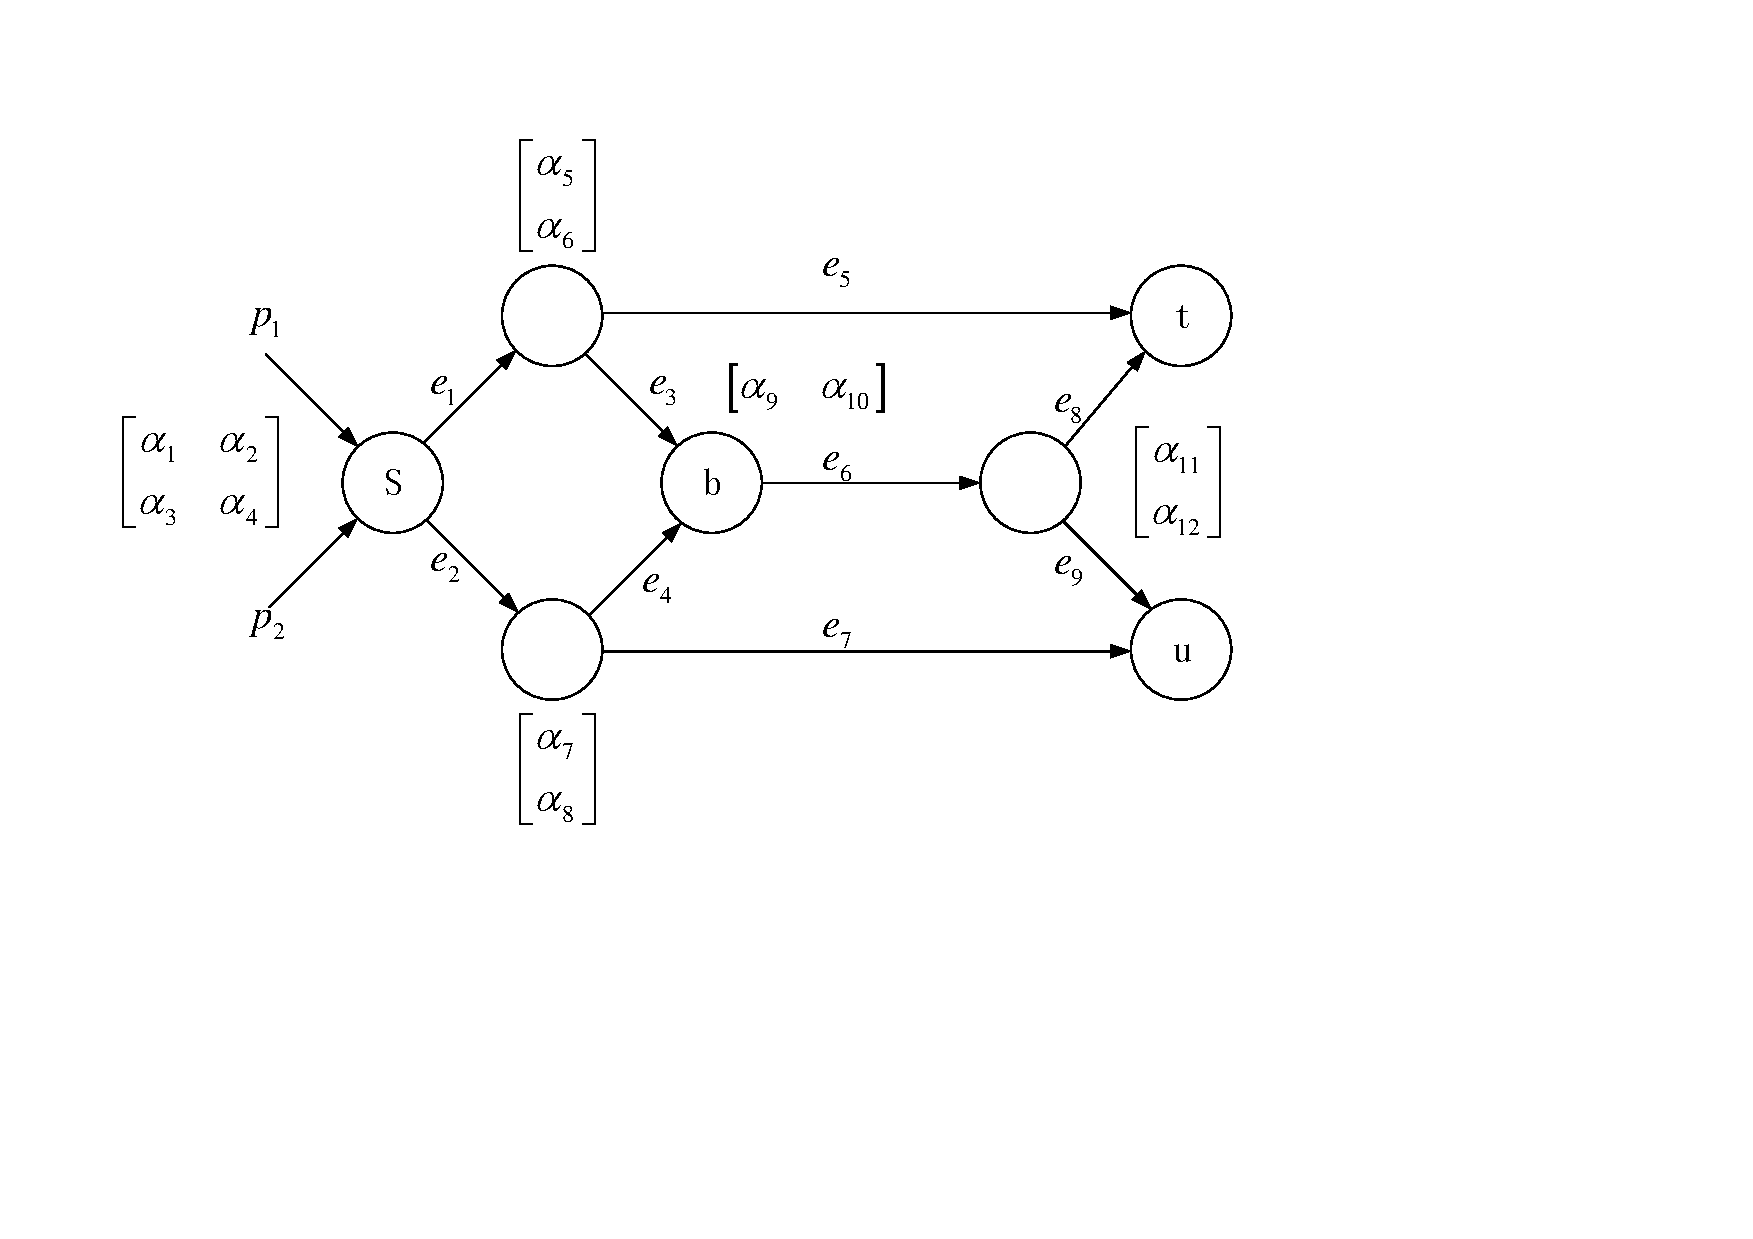
\includegraphics[width=6in]{figures/zhuanyi.pdf}
	\caption{标注了本地转移矩阵的蝶形网络}
	\label{ZHUANYI_EPS}
\end{figure}
\subsection{Network Coding 编码机制}
由于多径干扰、障碍物阻挡等原因,无线信道传输经常容易出错。链路层上比较著名的解决方法有前向纠错码( Forward Error Correction,FEC )和自动重传请求( Automatic Repeat Quest,ARQ )\textsuperscript{\cite{kurose2005computer}}。当错误是随机发生时,FEC可以有效地纠正报文的错误部分。FEC的优势是它不需要重传错误报文,也不会和TCP的原有机制产生冲突。FEC的缺点则是当链路质量很好地时候,会浪费带宽,而且会增加接收端CPU的计算和内存负担。同时,对于由于链路短暂断开导致的丢包,FEC也无能为力。当链路的丢包不是很频繁,还有传播时延不是很重要的时候,ARQ就比较有优势。然而,ARQ可能会与TCP的原有机制冲突\textsuperscript{\cite{kurose2005computer}}。为了有效控制丢包,有关学者将目光放在了基于FEC的编码机制上面,如纠删码( Erasure Coding )\textsuperscript{\cite{rizzo1997effective}}和网络编码\textsuperscript{\cite{Ahlswede2000,chou2003practical,algebraicapproach}}。
\par
网络中的数据包一般被看做是字节流。若干个数据包组成一个字节流,这个字节流被切分为$k$段,称为一个“\emph{generation}”\textsuperscript{\cite{chou2003practical}}。对于每一个\emph{generation},编码端使用随机线性编码产生$n$个经过编码的数据包。在目的节点,$n$个编码报文的任意$k$个独立数据包就足够恢复出原始数据包。换句话说,我们可以容忍网络中丢失$n-k$个报文。纠删码和网络编码的区别是前者只在源节点进行编码,而后者则在网络中的各个节点进行编码。实际上,纠删码可以看做是网络编码的特例。
\par
在恶劣的网络环境下,端到端的纠删码不足以实现可靠报文传输\textsuperscript{\cite{4753100}}。一些学者将网络编码应用于这些极具挑战性的网络中。和纠删码不同,网路的中间节点也会参与到编码中。在一些网络编码的实际应用中,“Batch Network Coding”是应用最为广泛的一种\textsuperscript{\cite{chachulski2007trading,algebraicapproach,chou2003practical,ho2003randomized,chen2009codecast,4015713}}。先介绍Batch Coding的相关原理。表\ref{SHUYU}是后面会用到的一些术语。
\begin{table}[htbp]
	\centering
	\caption{相关术语}
	\begin{tabularx}{350pt}{l|X}
		\toprule
		\textbf{名词} & \textbf{定义}\\
		\midrule
		Batch Coding & 每一个编码包会对同一个\emph{generation}里面的所有原始报文进行编码,只有\emph{generation}满秩之后才会进行编码或者解码\\
		\hline
		流水线编码 & 每当一个数据报文来之后,就会产生一个编码包,目的节点会逐步解出原始报文\\
		\hline
		\emph{generation} & 数据包的集合,作为编码和解码的整体\\
		\hline
		编码向量 & 反应组成某个编码数据包中各个原始数据包的系数\\
		\hline
		秩 & 线性独立的编码包的个数\\
		\hline
		编码冗余 & \emph{generation}的大小去除一个\emph{generation}生成的编码报文的个数得到的商\\
		\hline
		“Innovative”报文 & 一个可以增加秩的报文 \\
		\hline
		Delay & 目的站点的应用收到包的时间和包从源节点的应用产生的时间的差\\
		\bottomrule
	\end{tabularx}

\label{SHUYU}
\end{table}
\subsubsection[Batch Coding]{\textbf{Batch Coding}}
\par
假定在源节点有一个应用在不断产生同样大小的数据包\emph{$p_{1}$},\emph{$p_{2}$},\emph{$p_{3}$},$\dots$,。\emph{generation}的大小为$k$。第$i^{th}$个\emph{generation}产生的一个编码包可以被表示为:
\begin{equation}\label{eq24}
c = \sum\limits_{j = 1}^k {{e_j}{p_{i \times k + j}}}
\end{equation}
这里$e_{k}$是某个有限域$\mathbb{F}$中的一个元素,$i \times k$是在第$i$个\emph{generation}之前传输的的包的个数。每个数据包都被看做是在有限域$\mathbb{F}$上的一个向量,所有操作都是在有限域$\mathbb{F}$上进行。令$r$表示编码冗余度,$r  \ge 1$。对于每一个\emph{generation},源节点会产生$k \times r$个编码包。在目的节点,收到$k$个线性独立的包后,目的节点通过高斯消元解公式\ref{eq25},就可以恢复出原来$k$个数据包。
\begin{equation}\label{eq25}
\left[ {\begin{array}{*{20}{c}}
	{{c_1}}\\
	\vdots \\
	{{c_k}}
	\end{array}} \right] = \left[ {\begin{array}{*{20}{c}}
	{e_1^{\left( 1 \right)}}& \cdots &{e_k^{\left( 1 \right)}}\\
	\vdots & \ddots & \vdots \\
	{e_1^{\left( k \right)}}& \cdots &{e_k^{\left( k \right)}}
	\end{array}} \right]\left[ {\begin{array}{*{20}{c}}
	{{p_1}}\\
	\vdots \\
	{{p_k}}
	\end{array}} \right]
\end{equation}
\par
由于每个编码数据包都是同一个\emph{generation}的数据包的线性组合,在源节点就引入了一个延时。换句话说,同一个\emph{generation}里面前面的报文需要等后面的报文,直到这个\emph{generation}满秩后,才可进行编码。在目的节点处,同一个\emph{generation}的报文,要么都没解码,要么一个都解不出。
\par
为了刻画Batch Coding整个的时延,我们定义“delay”如下:接收端的应用收到报文的时间和源节点的应用产生报文的时间的差值。$t_{i}$表示源节点产生{\textbf{data}}\textsubscript{\textbf{i}}的时间,$t_{ci}$表示第$i$个编码包被发出去的时间。假定报文传输过程中的处理时延、传输时延、传播时延和排队时延都是常数,$d_{n}$表示网络中出现的时延的总和,$d_{c}$表示接收端的解码过程的时延,也为一个常数。假定一个\emph{generation}还有$k$个数据包,那么在无损信道中,传送数据包{\textbf{data}}\textsubscript{\textbf{i}}的时延为:
\begin{equation}\label{eq26}
{t_{c\left\lceil {{i \mathord{\left/
					{\vphantom {i k}} \right.
					\kern-\nulldelimiterspace} k}} \right\rceil *k}} - {t_i} + {d_n} + {d_c}
\end{equation}
\begin{figure}[htbp]
	\centering
	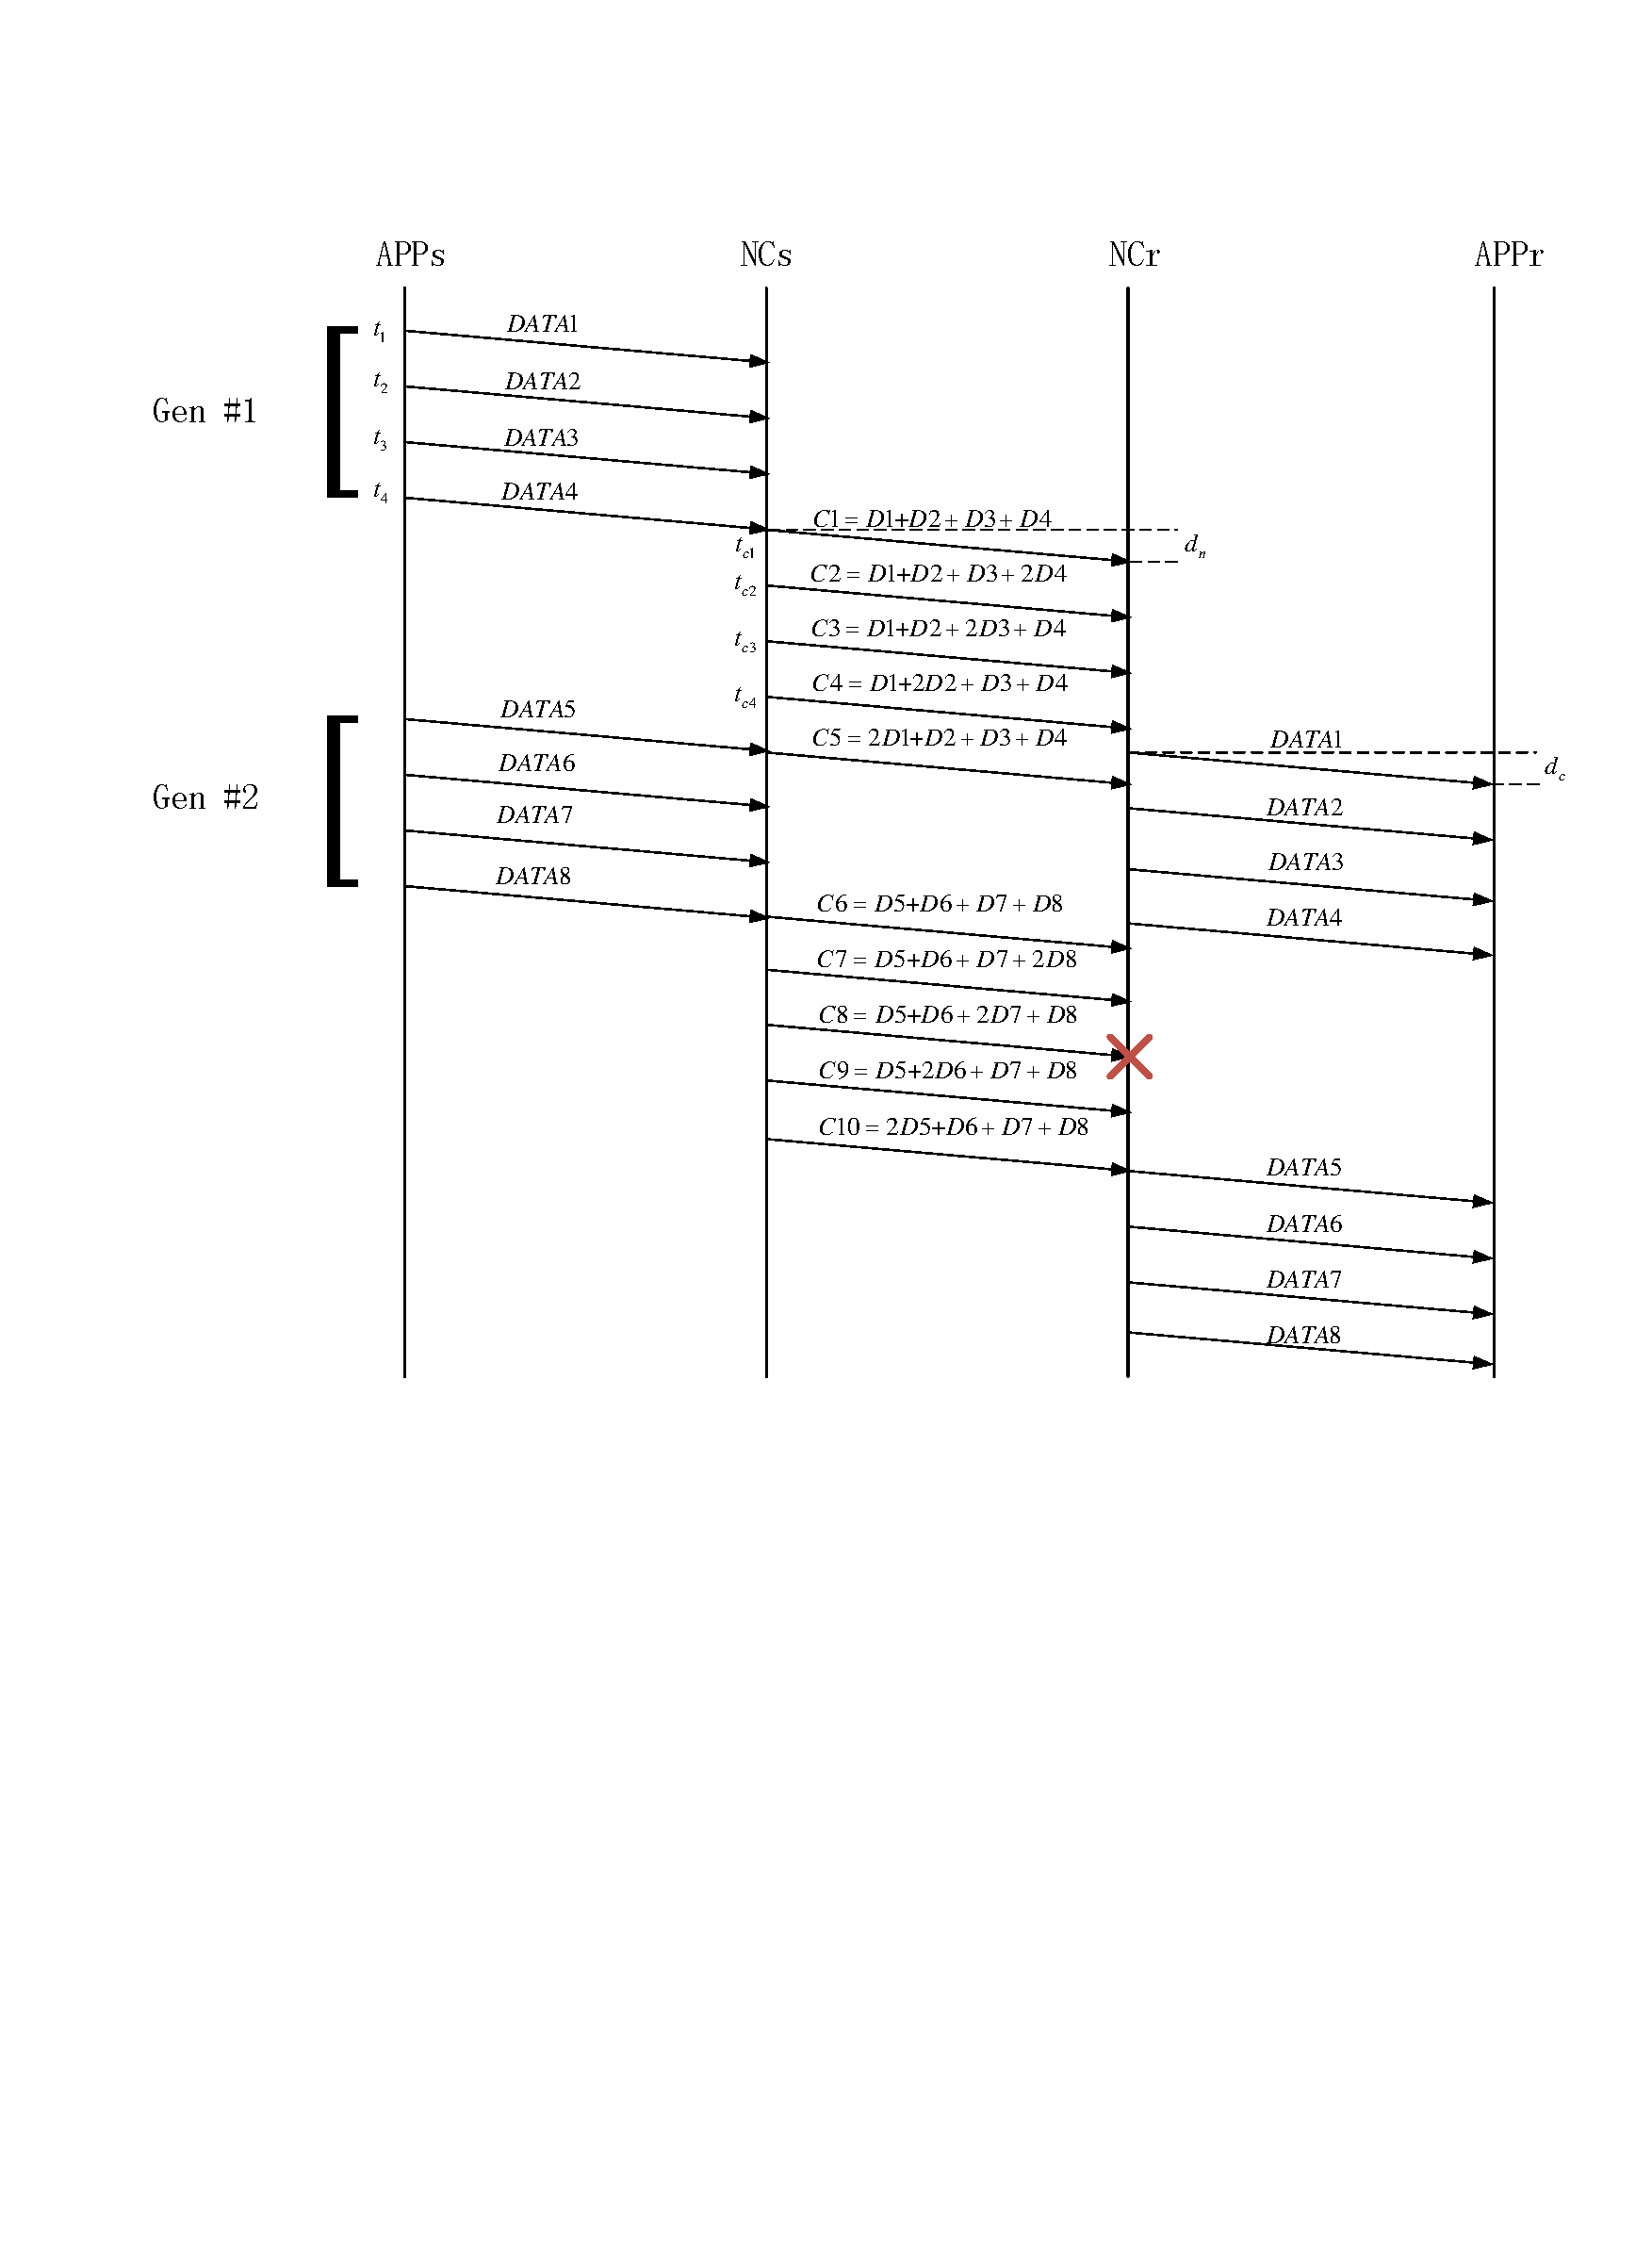
\includegraphics[width=6in]{figures/batch.pdf}
	\caption{Batch Coding 例子}
	\label{BATCHCODING_EPS}
\end{figure}
例如,在图\ref{BATCHCODING_EPS}中,传送\emph{data\textsubscript{1}}的时延为$t_{c4}-t_{1}+d_{n}+d_{c}$。这里\emph{generation}的大小为4,编码冗余为1.25.因此对于每个\emph{generation}来说,都会发送$k*r=5$个编码包。
\par
如果链路中出现丢包,接收端只需要收到4个线性独立的编码包就可以解出对应的\emph{generation}的所有原始数据报文。图\ref{BATCHCODING_EPS}中的“generation \# 2”描述了一个丢包被恢复,解码端成功解码的例子。然而如果冗余度不够补偿丢失的话,那么这个\emph{generation}就没有报文被解出来。如图\ref{BATCHUNDECODE_EPS},丢了$C4$和$C5$,接收端无法解码。
\begin{figure}[htbp]
\centering
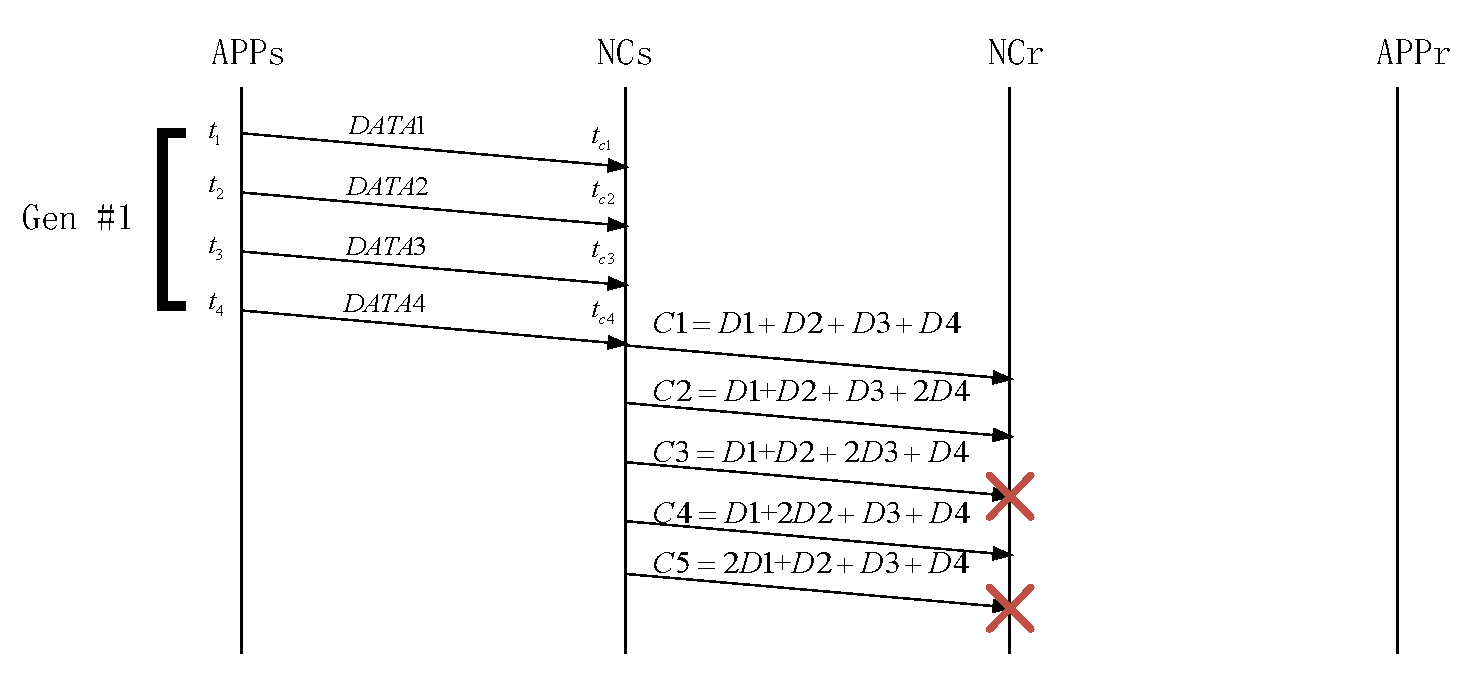
\includegraphics[width=6in]{figures/batchundecode.eps}
\caption{Batch Coding 例子}
\label{BATCHUNDECODE_EPS}
\end{figure}
\par
“Batch Network Coding”指的是这样一类编码:源节点和网络中的中间节点在同一个\emph{generation}上进行编码,目的节点只有在收到足够多的编码报文后,才能一次性解出这一个“\emph{generation}”中的所有原始报文。 
\par
Batch Network Coding有两个显著的缺点:首先,它引进了和\emph{generation}大小成比例的编解码时延,对于实时性要求比较高的应用来说,会限制\emph{generation}的大小,也就会降低编码的弹性;其次,只有当接收到足够多的线性独立的编码报文后,才可以解出一个\emph{generation}的所有报文,否则,整个\emph{generation}会被丢弃。
\par
文献\cite{chen2010pipeline}的作者针对Batch Network Coding的弱点提出了流水线网络编码( Pipeline  Network Coding )。
\subsubsection[Pipeline Coding]{\textbf{流水线编码}}\label{pipelinesec}
流水线编码旨在减少编解码时延,进而提高吞吐率。和Batch Coding不一样的是,流水线编码不需要等集满一个\emph{generation}大小的报文后才进行编码,与公式\ref{eq24}稍微不同,流水线编码的编码函数为:
\begin{equation}
c = \sum\limits_{j = 1}^m {{e_j}{p_{i \times k + j}}}
\end{equation}
其中,$m$为目前在编码缓存中的数据包个数。换句话说,如果收到一个原始报文,发送端基于目前收到的数据包立马执行一个编码函数。如果所有的编码包都依次正确地送到目的节点,那么目的节点可以构建如下的下三角矩阵:
\begin{equation}\label{eq28}
\left[ {\begin{array}{*{20}{c}}
	{{c_1}}\\
	\vdots \\
	{{c_k}}
	\end{array}} \right] = \left[ {\begin{array}{*{20}{c}}
	{e_1^{\left( 1 \right)}}&0& \cdots &0\\
	{e_1^{\left( 2 \right)}}&{e_2^{\left( 2 \right)}}&{}& \vdots \\
	\vdots &{}& \ddots &0\\
	{e_1^{\left( k \right)}}&{e_2^{\left( 2 \right)}}& \cdots &{e_k^{\left( k \right)}}
	\end{array}} \right]\left[ {\begin{array}{*{20}{c}}
	{{p_1}}\\
	\vdots \\
	{{p_k}}
	\end{array}} \right]
\end{equation}
上述方程可以逐步求解,而无需等待整个的\emph{generation}报文都集齐。例如,收到$c_{1}$,目的节点可以解码出$p_{1}$,以此类推。编码冗余的设计与Batch Coding略有不同。令$r$为编码冗余度,$r \ge 1$。对于每个数据包来说,$r - \left\lfloor r \right\rfloor $的概率产生$\left\lfloor r \right\rfloor + 1$个编码包,$1 - \left({r - \left\lfloor r \right\rfloor} \right)$的概率产生$r$个编码包。
\begin{figure}[htbp]
	\centering
	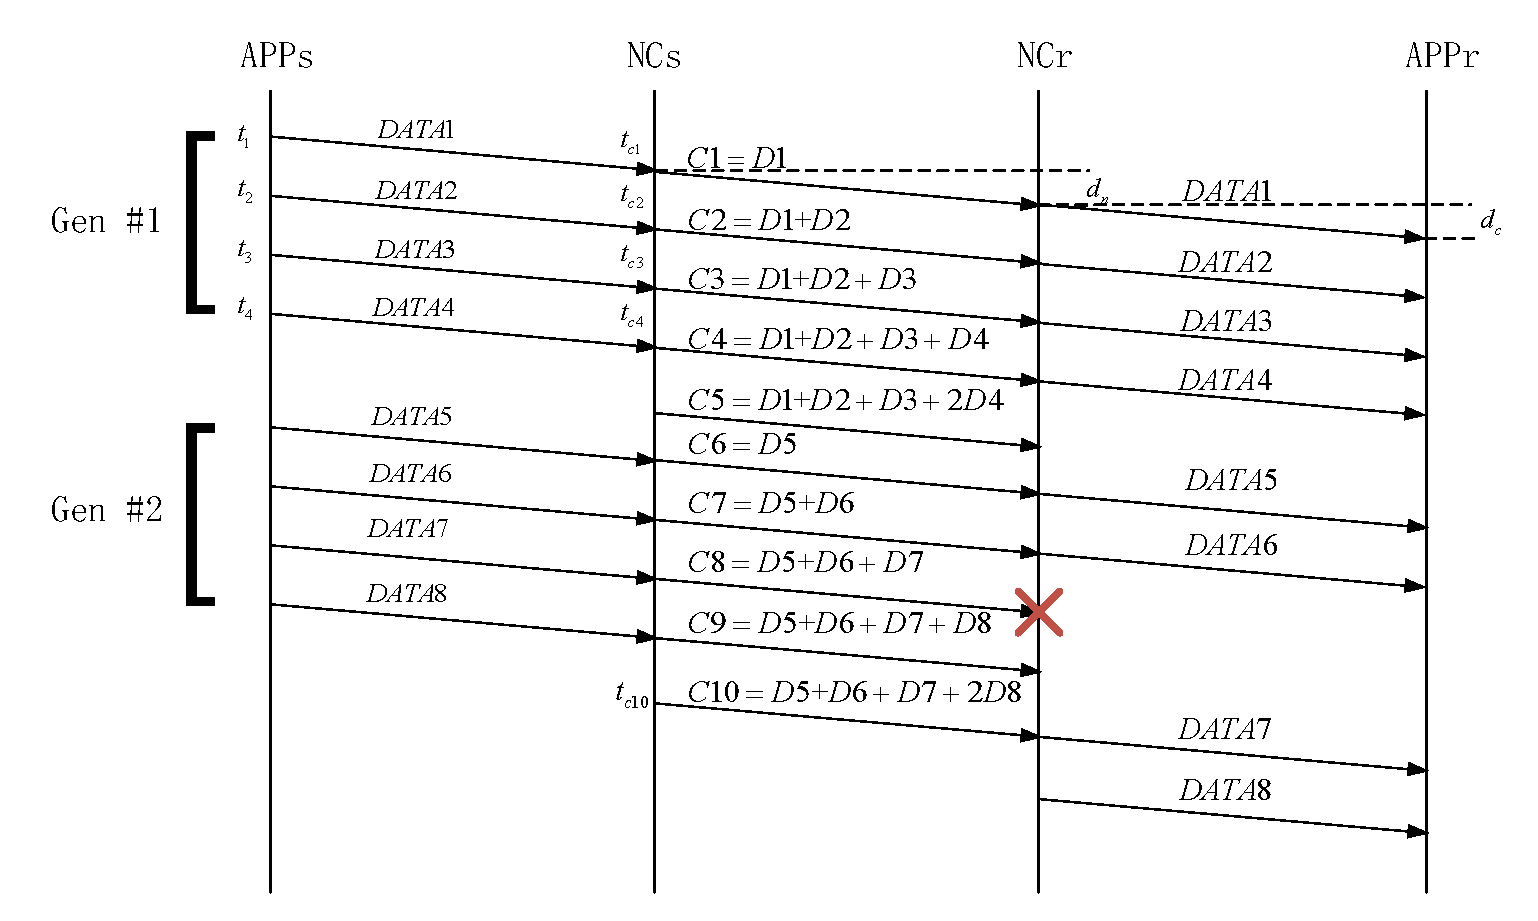
\includegraphics[width=6in]{figures/pipeline.eps}
	\caption{流水线编码}
	\label{LIUSHUIXIAN_EPS}
\end{figure}
\par
与前面分析Batch Coding时一样,我们让$t_{i}$表示源节点产生数据\textbf{data}\textbf{\textsubscript{i}}的时间,$t_{ci}$表示第$i$个编码数据包被发出去的时间。那么传送数据包\textbf{data}\textbf{\textsubscript{i}}的时延为$t_{ci} - t_{i}+d_{n}+d_{c}$。在大多数情况下,这比公式\ref{eq26}所表示的时延小多了。
\par
图\ref{LIUSHUIXIAN_EPS}展示了一个流水线编码的例子。这里\emph{generation}的大小为4,冗余度为1.25。当有一个原始数据包产生时,立马就编码得到一个编码包。同样地,在解码端,每当有一个“innovative”报文到来的时候,就可以立马解出一个原始报文。
\par
对于丢包的情况,图\ref{LIUSHUIXIAN_EPS}中\emph{Gen \# 2}中的$C8$丢失,目的节点在收到$C9$后,无法解出$DATA7$。这时候需要将undecoded packets存起来,等到冗余报文过来才可以解出原始报文,如图\ref{LIUSHUIXIAN_EPS}中的$C10$。Batch Coding的编解码流程如Algorithm\ref{algo1}和Algorithm\ref{algo2}:
\begin{algorithm}  
	\caption{Encoding Function}  
	\label{algo1}
	\KwIn{coding redundancy $r$,data packet \emph{data} from up-layer,$generation\_buffer\left[0,\dots,m,\dots \right]$,number of packets currently in \emph{generation buffer} $m-1$}  
	\KwOut{NONE}  
	Store $data$ to \emph{generation buffer}\;
	%%$i$ \leftarrow $0$ \;
	$i \leftarrow 0$\;
	\While{$i<num$}  
	{  
		\If{$\left(num-i<1 \wedge rand()\% 100 > num-i\right)$}  
		{  
			\Break\;
		} 
	Generate Coding Vector\;
	\For{$j=0;j \le m-1;j++$}
	{
		\If{$generation\_buffer[j]==NULL$}{$coding\_vector[j]=0$}
	}
	Encode packet\;
	Send Coded Packet to MAC layer\;
	%%$i$ \leftarrow $i+1$\;
	$i \leftarrow i+1$\;
}
\end{algorithm}

\begin{algorithm}  
	\caption{Decoding Function}
	\label{algo2}  
	\If{(not innovative(\emph{data}))}
	{
		Message\_Free(\emph{data})\;
		\Return;
	}
	Store \emph{data} to \emph{generation buffer}\;
	Gaussian\_Elimination(\emph{generation})\;
	\If{(decodable packets cause no reordering)}
	{
		Deliver to Transport(newly decodec data packets)\;
	}
\end{algorithm}

\section{TCP/NC协议}
\par
网络编码自出现以来就作为一种重要的改善网络性能,尤其是无线网络性能的工具。它的主要优势在于能够跨时间、跨流地将数据混合起来。这可以让在lossy信道中的数据传输更为健壮和高效。尽管如此,我们还是很少看见应用网络编码的实际例子,一个主要原因就是如何将网络编码很自然地加入到现有的网络体系中,而不与其冲突。
\par
Sundararajan等人在“Network Coding Meets TCP”\textsuperscript{\cite{Sundararajan2009}}一文中提出编码TCP协议( TCP/NC),用于提高标准TCP协议在无线网络环境下的性能。其通过在TCP层和IP层之间添加一个网络编码层来掩盖lossy信道中出现的随机丢包。与以往一些学者在改进TCP在无线网络下性能的工作不同的是,TCP/NC不需要对原有的OSI协议栈做出修改。TCP/NC可以很优雅地与标准TCP协议,IP协议,链路层的协议一起工作,不会与原有协议的机制冲突,适合大规模地部署在现有互联网体系中。在详细介绍TCP/NC协议之前,先引入\emph{ACK on degree of freedom}这个概念。
\subsection{ACK on degree of freedom}\label{ackondegree}
现有的很多可靠传输协议都有ACK这个机制,如TCP,ARQ等。接收方通过回复发送方ACK来让发送方了解自己收到了哪些数据。如果在没有应用编码的网络中,那么接收端在收到原始报文后就可以回给发送方ACK;如果在应用了网络编码的网络中,如文献\cite{Lun2008On},接收端需要在收到若干个数据包后,对整体进行解码恢复原始数据包,才会回复ACK,亦如第二章介绍的Batch Coding,其缺点是传送数据包的时延较长。针对Batch Coding的缺点,文献\cite{chen2010pipeline}提出了流水线编码( Pipeline  Coding ),但是在丢包网络中也会存在ACK延迟的问题。图\ref{LIUSHUIXIAN_EPS}中的$DATA7$和$DATA8$需要等到收到$C10$后才可以解出,进而回给发送端ACK。ACK的延迟不仅会影响吞吐率,还会影响发送端的编码队列的长度。直觉来说,编码端只有在收到某个数据包的ACK后,才会将其从编码缓存中删除。例如,源节点有$n$个数据包( 每个数据包看做是有限域$\mathbb{F}$上的向量 ),分别是$p_{1}$,$p_{2}$,$\dots$,$p_{n}$。经过编码,依次发出去$n$个编码包,分别是$p_{1}$,$\left(p_{1}+p_{2}\right)$,$\left(p_{2}+p_{3}\right)$,$\dots$,$\left(p_{n-1}+p_{n}\right)$。由于网路质量差,第一个包$p_{1}$丢了,接收端只收到$\left(p_{1}+p_{2}\right)$,$\left(p_{2}+p_{3}\right)$,$\dots$,$\left(p_{n-1}+p_{n}\right)$。接收端尽管收到了$n-1$个编码包,但一个也无法解出来,也就无法给源节点确认ACK。可靠传输要求发送端在没收到接收端确认ACK时必须把$p_{1}$,$p_{2}$,$\dots$,$p_{n}$都放入缓存队列。我们可以看到这个队列此时的长度长达$n$。
\par
针对以上问题,文献\cite{4595268}首次提出了“ACK on degree of freedom”的概念。在介绍“ACK on degree of freedom”之前,我们先引入一个定义。
\begin{myDef}[Seeing a packet]\label{df26}
	如果一个节点根据现有的信息可以计算出如\textbf{\emph{$\left(p+q\right)$}}形式的线性组合,那么我们就说这个节点“\textbf{see packet \emph{$p$}}”。其中\textbf{$q$}本身就是只包含序号比$p$大的报文的线性组合。解码出某个报文也算作是“seeing a packet”,此时\textbf{$q=0$}。

\end{myDef}
\par
直觉告诉我们,如果目的节点已经\emph{see packet $p$},那么发送端那边在产生编码包的时候,就不必将数据包$p$再囊括进去了。换句话说,发送端可以将数据包$p$从编码缓存中移除。接收端如果后面接收到足够的信息,将$q$解出来,那么$p$自然就解出来了。因此,接收端如果已经\emph{see packet $p$},那么其可以直接向发送端回复ACK,表示自己已经收到了报文$p$,通知发送端那边将报文$p$从编码缓存中移除。
\par
表\ref{tab:drop-when-seen}展示的就是\emph{ACK on degree of freedom} 的一个例子。在时隙1时,发送端发送了报文$p_{1}$,$p_{1}$在链路中丢失了,目的节点\emph{A}没有收到;在时隙2时,由于\emph{A}没有发送对报文$p_{1}$的ACK,所以源节点发送缓存为$p_{1}$和$p_{2}$,接着发送端对$p_{1}$和$p_{2}$进行异或,得到编码包,发出去。目的节点收到了编码包,虽然无法解出$p_{1}$和$p_{2}$,但根据定义\ref{df26},\emph{A}看到了$p_{1}$。因此,\emph{A}回复源节点一个ACK,让源节点将$p_{1}$从编码缓存中移除。我们可以看到,在时隙3时,源节点的发送缓存只有$p_{2}$和$p_{3}$,和前面一样,源节点发送编码包$p_{2} \oplus p_{3}$。这一次\emph{A}正确地收到了,\emph{A}看到了$p_{1}$和$p_{2}$,但还是无法解出它们。我们看到,一直到时隙5,\emph{A}都没有解出一个报文,但看到的报文( seen packet )有$p_{1}$,$p_{2}$,$p_{3}$。源节点在时隙6发送了$p_{4}$,导致$p_{5}$被看到,然后在时隙7发送了$p_{5}$,让\emph{A}解出了所有报文。
\begin{table}[htbp]  
	\centering  
	\fontsize{6.5}{8}\selectfont  
	\begin{threeparttable}  
		\caption{\emph{ACK on degree of freedom} 例子}  
		\label{tab:drop-when-seen}  
		\begin{tabular}{c|c|c|c|c|c}  
			\toprule  
			\multirow{2}{*}{Time} &\multirow{2}{*}{Sender's queue} & \multirow{2}{*}{Transmitted packet} & \multirow{2}{*}{Channel state}&  
			\multicolumn{2}{c}{ Destination Node \emph{A}}\cr  
			\cmidrule(lr){5-6}  
			\hspace{1cm}&\hspace{1cm}&\hspace{1cm}&\hspace{1cm}&Decoded&Seen but not decoded\cr  
			\midrule  
			1&$p_{1}$&$p_{1}$&$\nrightarrow A$&\hspace{1cm}&\hspace{1cm}\cr
			\hline  
			2&$p_{1}$,$p_{2}$&$p_{1} \oplus p_{2}$&$\rightarrow A$&\hspace{1cm}&$p_{1}$\cr 
			\hline 
			3&$p_{2}$,$p_{3}$&$p_{2} \oplus p_{3}$&$\rightarrow A$&\hspace{1cm}&$p_{1}$,$p_{2}$\cr
			\hline  
			4&$p_{3}$,$p_{4}$&$p_{3} \oplus p_{4}$&$\nrightarrow A$&\hspace{1cm}&$p_{1}$,$p_{2}$\cr
			\hline  
			5&$p_{3}$,$p_{4}$,$p_{5}$&$p_{3} \oplus p_{4} \oplus p_{5}$&$\rightarrow A$&\hspace{1cm}&$p_{1}$,$p_{2}$,$p_{3}$\cr
			\hline  
			6&$p_{4}$&$p_{4}$&$\rightarrow A$&$p_{4}$&$p_{1}$,$p_{2}$,$p_{3}$,$p_{5}$\cr
			\hline
			7&$p_{5}$&$p_{5}$&$\rightarrow A$&$p_{1}$,$p_{2}$,$p_{3}$,$p_{4}$,$p_{5}$&\hspace{1cm}\cr    
			\bottomrule  
		\end{tabular}  
	\end{threeparttable}  
\end{table}  
\par
总结一下,\emph{ACK on degree of freedom}就是说我不再对原始数据包进行ACK确认,而是确认\emph{自由度}。只要接收端看到了某个报文( see a packet ),即使没有解出来,依然可以恢复发送端对seen packet的确认。
\subsection{TCP/NC架构分析}
文献\cite{4298308}在对网络编码与现有协议结合中可能出现的问题作出过分析,具体到TCP来说,就是寻找一种能够与现有的TCP的滑动窗口兼容的编码机制。本文第\ref{pipelinesec}小节介绍的Pipeline Coding就与TCP的滑动窗口很相似。与文献\cite{chou2003practical,chachulski2007trading}中用到的Batch Coding不同,Pipeline Coding的编码过程是渐进性的。每下来一个原始报文,就产生一个或者多个编码包。
\par
TCP可靠传输的背后思想是使用Acknowledgements对按序到来的数据包进行确认,同时发送端使用ACK来进行拥塞控制。对于使用网络编码来说,这个机制需要做点改变。其原因在于使用网络编码后,接收端收到的不再是原始数据包,而是原始数据包的线性组合( 这里仅针对线性网络编码 )。一旦收到足够多的线性组合,就可以解码得到原始数据包。标准TCP中“\emph{按序到达的报文}”这个概念缺失了。现有的ACK机制不允许我们确认还未解码的数据包。本文第\ref{ackondegree}小节所讲到的\emph{ACK on degree of freedom}概念值得借鉴。绝大多数情况,接收端收到的线性组合报文都会给接收端带来新信息( 在有限域$\mathbb{F}$下有可能出现非线性独立的编码包 ),也就是自由度( 将编码数据包看做是向量 )。TCP/NC对于收到的编码包产生的自由度回复ACK,而不管这个新来的包是否让接收端解出了一个包。
\par
TCP/NC在传输层和网络层引入了一个Network Coding Layer( NC层 ),如图\ref{TCPNC_EPS},并再次利用了标准TCP的拥塞控制机制,也就是正在传输的报文字节数和ACK序号之间的差值不能超过拥塞窗口的值。TCP/NC在原有协议栈的机制上作出了两点改变:首先,无论何时发送端被允许发送数据包的时候,它发送的是拥塞窗口的报文的线性组合;第二,接收端对于其收到的每个自由度回复ACK,而不是对原始报文回复ACK。
\par
\begin{figure}[htbp]
	\centering
	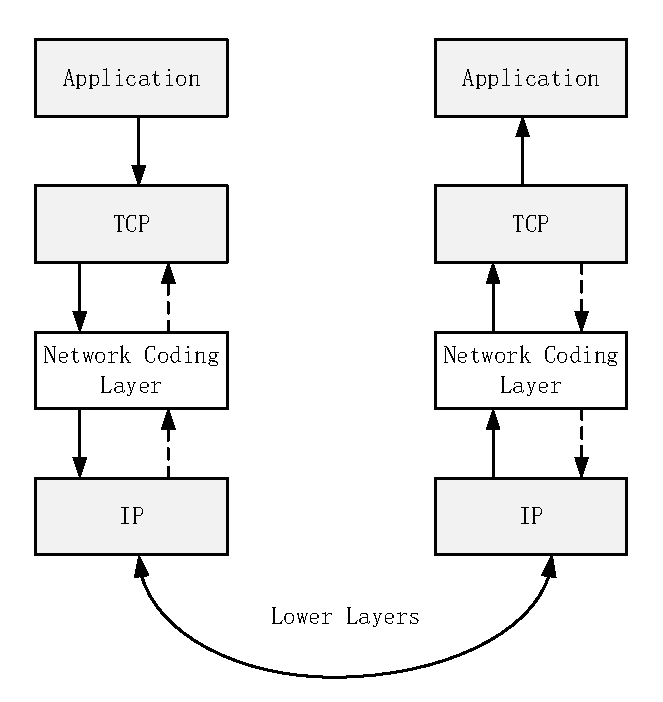
\includegraphics[width=3in]{figures/tcpnc.eps}
	\caption{TCP/NC协议架构}
	\label{TCPNC_EPS}
\end{figure}
\par
在发送端,NC层缓存从TCP层下来的报文
\textbf{使用~\LaTeX{}~进行科学排版的另一大优势就是可以灵活地在文章中插入矢量绘图},虽然在Word软件也支持插入同为Microsoft Office套件的Visio编辑的矢量图,然而Word其对其余主流矢量图格式(如.pdf, .eps等文件)的支持并不理想。图\ref{SWJTU_LOGO_PNG}和图\ref{SWJTU_LOGO_PDF}分别示出了位图格式和矢量格式的西南交通大学校徽\footnote{请注意,文中所使用的西南交通大学校徽文件中,位图版为采西南交通大学官方提供的校徽LOGO文件,矢量版校徽为模板作者通过软件自行勾勒得出,非官方的正式版,请不要在正式场合使用。},可以看出在放大比率为200\%的时候,位图校徽的边缘开始出现模糊的情形。与此同时,\textbf{由于矢量图是一种基于纯数学公式语言的绘图,采用矢量图制作的插图能够保证成像不会因为放大而失真同时保证很小的文件大小}。

\par
需要注意的是,并非所有的插图都适合采用矢量格式,尤其是照片之类的图片,通常情况下适宜采用.png或者.jpeg等位图格式;\textbf{而系统框图、曲线图、概念流程图等,则以采用矢量图格式为佳。}

\par
目前,主流的商业矢量插画绘制软件以ADOBE公司的Illustrator以及Corel公司的CorelDRAW为主,不过受制于其售价,一般学生用户可以使用一些免费的矢量图编辑软件,例如Inkscape\footnote{Inkscape官方网站:\url{https://inkscape.org/en/}},作为一款矢量图绘制的利器,其功能已经能够基本满足正常的需,深受广大用户的喜爱。
\section{本章小结}

